\documentclass[10pt,a4paper]{article}
\usepackage[margin=21mm,headheight=15pt]{geometry}
\usepackage[T1]{fontenc}
\usepackage{lmodern,amsmath,amssymb,tikz,graphicx,hyperref,fancyhdr,enumitem}
\usetikzlibrary{arrows.meta,positioning,calc,decorations.pathmorphing}
\definecolor{ink}{RGB}{20,53,78}
\hypersetup{colorlinks=true,urlcolor=ink,linkcolor=ink}
\setlength{\parindent}{0pt}\setlength{\parskip}{5pt}
\emergencystretch=3em
\pagestyle{fancy}\fancyhf{}\fancyfoot[C]{\thepage}
\renewcommand{\headrulewidth}{.3pt}
\newcommand{\task}[2]{\par\medskip{\color{ink}\Large\bfseries #1. #2}\par\smallskip}
\newcommand{\answer}{\par\smallskip\textbf{Worked reasoning.} }
\setlist[enumerate]{label=\textbf{(\alph*)},leftmargin=7mm,itemsep=7pt}
\begin{document}
\fancyhead[L]{\small Control of Dynamical Systems}
\fancyhead[R]{\small Laboratory 06}
{\color{ink}\LARGE\bfseries Laboratory 06}\par
{\large Gain selection with a third-order actuator}\par
\textbf{Worked solutions -- five integrated problems}\par
{\small\textbf{Evidence boundary.} Original hypothetical scenarios. Derive, calculate and justify decisions; every numerical record is synthetic. Figures are conceptual and not to scale.}
\smallskip\textbf{Shared nominal data.} Nominal unity negative-feedback loop: $G(s)=1/[s(s+2)(s+6)]$ and scalar controller $K$. The positioning-axis picture illustrates a possible application; the normalized coefficients are stipulated.
\task{1}{A position actuator with an identified aggregate model}
The sketch shows a possible motor-driven carriage. Its normalized plant $1/[s(s+2)(s+6)]$ is stipulated as an aggregate teaching model; the poles are not inferred from the drawing dimensions.
\begin{center}\resizebox{\ifdim\width>.98\linewidth.98\linewidth\else\width\fi}{!}{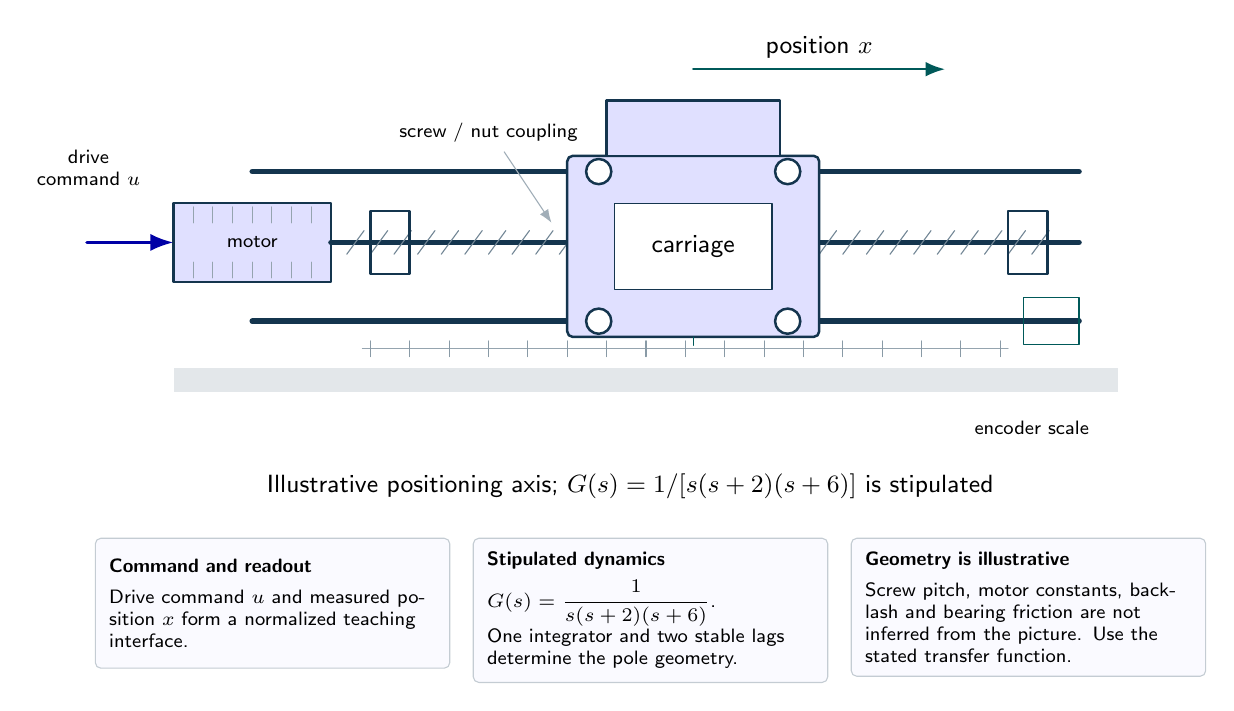
\begin{tikzpicture}[
font=\sffamily\small,>=Latex,line cap=round,line join=round,
wall/.style={draw=ink,line width=1.2pt,fill=blue!5},
water/.style={fill=cyan!25,draw=none},
metal/.style={draw=ink,fill=blue!12,line width=.9pt},
flow/.style={->,draw=blue!65!black,line width=1.2pt},
heat/.style={->,draw=orange!85!black,line width=1.1pt},
measure/.style={->,draw=teal!70!black,line width=.9pt},
dim/.style={<->,draw=ink!65,line width=.6pt},
spring/.style={draw=ink,decorate,decoration={coil,aspect=.5,segment length=4pt,amplitude=3pt}},
wire/.style={draw=ink,line width=1pt},
lab/.style={align=center,font=\sffamily\small},
smalllab/.style={align=center,font=\sffamily\scriptsize}]

\fill[ink!12](1,.5)rectangle(13,.8);
\draw[ink,line width=2pt](2,1.4)--(12.5,1.4)(2,3.3)--(12.5,3.3);
\draw[metal](1,1.9)rectangle(3,2.9);
\node[smalllab]at(2,2.4){motor};
\draw[ink,line width=2pt](3,2.4)--(12.5,2.4);
\foreach \x in {3.2,3.5,...,12.2}{\draw[ink!60](\x,2.25)--++(.22,.3);}
\draw[metal,rounded corners=2pt](6,1.2)rectangle(9.2,3.5);
\draw[fill=white,draw=ink](6.6,1.8)rectangle(8.6,2.9);
\node[lab]at(7.6,2.35){carriage};
\draw[metal](6.5,3.5)rectangle(8.7,4.2);
\draw[measure](7.6,4.6)--(10.8,4.6)node[midway,above]{position $x$};
\draw[flow](-.1,2.4)--(1,2.4);
\node[smalllab,anchor=east]at(.7,3.35){drive\\command $u$};
\draw[teal!70!black](11.8,1.1)rectangle(12.5,1.7);
\node[smalllab]at(11.9,.05){encoder scale};
\node[lab]at(6.8,-.7){Illustrative positioning axis; $G(s)=1/[s(s+2)(s+6)]$ is stipulated};
% REFINED EQUIPMENT DETAILS

% Guide bearings, screw supports and a scale tied to the carriage coordinate.
\foreach \x in {6.4,8.8}{\draw[metal,fill=white](\x,1.4)circle(.16)(\x,3.3)circle(.16);}
\draw[metal,fill=none](3.5,2)rectangle(4,2.8);\draw[metal,fill=none](11.6,2)rectangle(12.1,2.8);
\draw[ink!45](3.4,1.05)--(11.6,1.05);
\foreach \x in {3.5,4,...,11.5}{\draw[ink!50](\x,.95)--(\x,1.15);}
\draw[teal!70!black,densely dashed](7.6,1.2)--(7.6,1.05);
\foreach \x in {1.25,1.5,...,2.75}{\draw[ink!45](\x,1.95)--(\x,2.15)(\x,2.65)--(\x,2.85);}
\node[smalllab]at(5,3.8){screw / nut coupling};
\draw[ink!40,->](5.2,3.55)--(5.8,2.65);

\node[draw=ink!25,fill=blue!2,rounded corners=2pt,anchor=north west,text width=4.15cm,minimum height=1.65cm,inner sep=5pt,align=left,font=\sffamily\scriptsize]at(0.0,-1.35){\textbf{Command and readout}\\[3pt]Drive command $u$ and measured position $x$ form a normalized teaching interface.};
\node[draw=ink!25,fill=blue!2,rounded corners=2pt,anchor=north west,text width=4.15cm,minimum height=1.65cm,inner sep=5pt,align=left,font=\sffamily\scriptsize]at(4.8,-1.35){\textbf{Stipulated dynamics}\\[3pt]$G(s)=\dfrac{1}{s(s+2)(s+6)}$.\\One integrator and two stable lags determine the pole geometry.};
\node[draw=ink!25,fill=blue!2,rounded corners=2pt,anchor=north west,text width=4.15cm,minimum height=1.65cm,inner sep=5pt,align=left,font=\sffamily\scriptsize]at(9.6,-1.35){\textbf{Geometry is illustrative}\\[3pt]Screw pitch, motor constants, backlash and bearing friction are not inferred from the picture. Use the stated transfer function.};
\end{tikzpicture}
}\par{\small A motorized positioning axis illustrates the role of the integrator and two stable lags. The normalized transfer function is specified as a teaching model; the pictured dimensions do not identify its coefficients.}\end{center}
\begin{enumerate}
\item Consider unity negative feedback with loop $L(s)=K/[s(s+2)(s+6)]$, $K>0$. Derive the reference transfer function, characteristic polynomial and open-loop poles and zeros.
\answer The reference transfer is $T=L/(1+L)=K/[s(s+2)(s+6)+K]$. Expanding the product gives the characteristic polynomial $p=s^3+8s^2+12s+K$. The open loop has poles at 0, $-2$ and $-6$ and no finite zeros. Closed-loop poles depend on K; the open-loop poles are their limiting locations as $K\to0^+$.
\item Construct the cubic Routh first column. Find the full strictly stable positive-gain interval and classify its endpoints.
\answer The first column is $1,8,(96-K)/8,K$. All terms are positive exactly when $0<K<96$. At $K=0$, one pole is at the origin, so the system is not asymptotically stable. At $K=96$, the polynomial factors as $(s+8)(s^2+12)$ and has an imaginary pair. Both endpoints are excluded. Positive polynomial coefficients alone would miss the upper gain restriction.
\item A numerical step plot appears bounded for $K=97$ over a short interval. Use the algebraic result to decide whether this is sufficient evidence of stability and specify a decisive numerical check.
\answer For $K=97$, the Routh first column is $1,8,-1/8,97$, giving two sign changes and two right-half-plane poles. A short trajectory cannot override this conclusion. Compute all characteristic roots or the state eigenvalues and report their real parts; then extend the simulation with a generic initial perturbation. The duration and excitation can hide slowly growing modes, whereas the polynomial test classifies the nominal linear system.
\end{enumerate}

\newpage
\task{2}{Following branches through a breakaway}
Use the open-loop pole map to construct the locus geometrically, then verify the repeated-pole event algebraically. Reject stationary points that belong to the wrong gain sign.
\begin{enumerate}
\item Determine the positive-gain real-axis root-locus segments, asymptote centroid and asymptote angles. Explain how many branches reach infinity.
\answer A real point belongs to the positive-gain locus when the number of real poles and zeros to its right is odd. The segments are $(-\infty,-6)$ and $(-2,0)$. With three poles and no finite zeros, all three branches go to infinity. The centroid is $(0-2-6)/3=-8/3$, and angles are $(2q+1)180^\circ/3$: $60^\circ$, $180^\circ$ and $300^\circ$. The two rightward asymptotes are consistent with loss of stability at high gain.
\item Find the stationary points of $K(s)=-s(s+2)(s+6)$ on the real axis. Select the positive-gain breakaway point and calculate its gain.
\answer Differentiate: $dK/ds=-(3s^2+16s+12)=0$. The candidates are $s=(-8\pm2\sqrt7)/3$. Only $s_b=(-8+2\sqrt7)/3\approx-0.902832$ lies on the positive-gain segment $(-2,0)$. Substituting into $K(s)$ gives $K_b\approx5.04904$. The other candidate lies between $-6$ and $-2$, where positive-gain locus points are absent and its calculated gain is negative. Stationarity alone does not establish a valid breakaway.
\item At the valid breakaway, determine the third pole without solving another cubic. Check the repeated-pole factorization against the coefficient of $s^2$.
\answer The sum of all three roots is always $-8$. At the repeated pole $s_b=(-8+2\sqrt7)/3$, the remaining pole is $s_3=-8-2s_b=(-8-4\sqrt7)/3\simeq-6.19434$. Thus $p(s)=(s-s_b)^2(s-s_3)$ at $K=K_b$. Its $s^2$ coefficient is $-(2s_b+s_3)=8$, providing an independent check on branch selection and the repeated-root calculation.
\end{enumerate}

\newpage
\task{3}{Boundary oscillations and feedback-sign mistakes}
Classify the nominal loop at both stability boundaries and after reversing the controller sign. Distinguish input--output cancellation from decay of internal states.
\begin{center}\resizebox{\ifdim\width>.98\linewidth.98\linewidth\else\width\fi}{!}{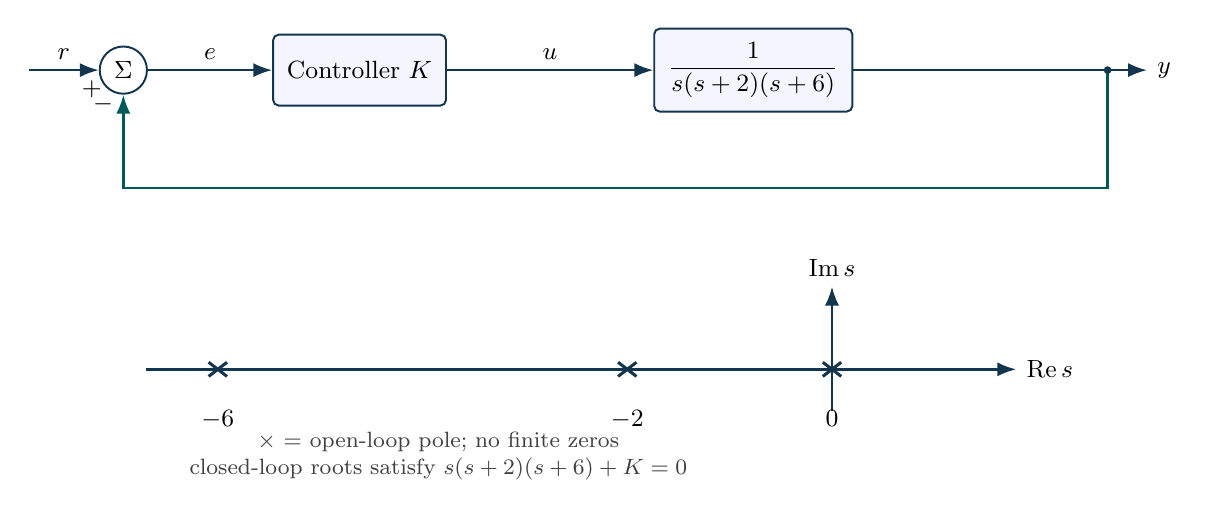
\begin{tikzpicture}[x=1cm,y=1cm,>=Latex,font=\small,
block/.style={draw=ink,fill=blue!4,rounded corners=2pt,minimum height=9mm,align=center,line width=.7pt,inner sep=5pt},
sum/.style={circle,draw=ink,fill=white,minimum size=6mm,inner sep=0pt,line width=.7pt},
sig/.style={->,draw=ink,line width=.85pt},
fb/.style={->,draw=teal!70!black,line width=.85pt},
dist/.style={->,draw=orange!75!black,line width=.85pt},
tap/.style={circle,fill=ink,inner sep=1.4pt},
note/.style={font=\footnotesize,align=center,text=black!75}]

\node[sum](e)at(1,1.8){$\Sigma$};
\node[block](k)at(4,1.8){Controller $K$};
\node[block](p)at(9,1.8){$\dfrac{1}{s(s+2)(s+6)}$};
\draw[sig](-.2,1.8)--node[above]{$r$}node[pos=.9,below]{$+$}(e);
\draw[sig](e)--node[above]{$e$}(k);
\draw[sig](k)--node[above]{$u$}(p);
\draw[sig](p)--(14,1.8)node[right]{$y$};
\draw[fb](13.5,1.8)--(13.5,.3)--(1,.3)--node[pos=.9,left]{$-$}(e);
\fill[ink](13.5,1.8)circle(1.4pt);
\begin{scope}[shift={(10,-2)},x=1.3cm,y=.75cm]
\draw[sig](-6.7,0)--(1.8,0)node[right]{$\operatorname{Re}s$};
\draw[sig](0,-.7)--(0,1.4)node[above]{$\operatorname{Im}s$};
\foreach \v in {-6,-2,0}{\draw[ink,line width=1.1pt](\v-.09,-.12)--(\v+.09,.12)(\v-.09,.12)--(\v+.09,-.12);\node[below=4mm]at(\v,0){$\v$};}
\end{scope}
\node[note]at(5,-3.1){$\times$ = open-loop pole; no finite zeros\\closed-loop roots satisfy $s(s+2)(s+6)+K=0$};

\end{tikzpicture}
}\par{\small Unity negative feedback and the open-loop pole map. Pole symbols provide the starting geometry for the root-locus exercises.}\end{center}
\begin{enumerate}
\item At the upper stability boundary, calculate the oscillation frequency and period and the third pole. Explain whether a bounded-looking oscillation over a finite simulation interval establishes asymptotic stability.
\answer At $K=96$, $p=(s+8)(s^2+12)$. The pair is $\pm j\sqrt{12}$, with angular frequency $2\sqrt3\approx3.46410$ rad/s and period $2\pi/\sqrt{12}=\pi/\sqrt3\approx1.81380$ s. The third pole is $-8$. The undamped pair does not decay. A finite plot may look bounded even at a marginal boundary or during slowly growing instability, so pole analysis is required for asymptotic stability.
\item For $K<0$, prove that at least one real closed-loop pole is positive without using a root solver. Relate the result to the feedback sign.
\answer The real polynomial satisfies $p(0)=K<0$ and $p(s)\to+\infty$ as $s\to+\infty$. Continuity therefore guarantees a positive real root. The closed loop is unstable for every negative K. A sign reversal turns the intended feedback action into reinforcement for the low-frequency positive plant gain. This argument establishes instability without needing the other two poles.
\item At $K=0$, the reference-to-output transfer has zero numerator. Does that imply every internal state converges to zero? Explain using the unreduced plant modes and nonzero initial conditions.
\answer No. At $K=0$, the plant retains modes $0,-2,-6$; the zero mode does not decay. The reference is disconnected, so the zero-state transfer from reference may be identically zero while an initial displacement persists. Internal asymptotic stability must be checked in the state dynamics or unreduced characteristic equation. Neither a zero transfer nor a finite plot with no excitation proves decay of all internal modes.
\end{enumerate}

\newpage
\task{4}{A tracking specification with gain uncertainty}
Proportional gain must satisfy both a ramp-error specification and strict stability. Treat these inequalities jointly rather than increasing gain until the plot looks acceptable.
\begin{enumerate}
\item For stable K, derive the position and velocity error constants. Find the unit-step and unit-ramp steady errors at $K=24$. State the stability qualification.
\answer The open-loop integrator makes $K_{pos}=\lim_{s\to0}L(s)=\infty$ and $K_v=\lim_{s\to0}sL(s)=K/12$. Thus a unit step has zero nominal steady error and a unit ramp has $e_\infty=12/K$. At $K=24$, these are zero and 0.5. The final-value reasoning applies because $24$ lies inside $(0,96)$. Applying the same formulas to an unstable closed loop would not yield a valid final error.
\item Require unit-ramp error no larger than 0.1 using only positive proportional K. Combine the error and stability conditions. What design conclusion follows?
\answer The ramp condition $12/K\le0.1$ requires $K\ge120$. Strict stability requires $K<96$, so no gain satisfies both. Even the excluded marginal value $K=96$ would give the formal ramp error 0.125. The architecture needs modification, such as dynamic compensation, rather than a larger proportional gain. This conclusion concerns the stated linear model and reference class.
\item Relax the allowed unit-ramp error to 0.15 and select nominal $K=84$. If actual gain is $84(1+\delta)$ with $|\delta|\le\varepsilon$, find the largest symmetric uncertainty bound that preserves both requirements.
\answer The relaxed tracking condition is $K\ge12/0.15=80$, and stability requires $K<96$. Therefore $84(1-\varepsilon)\ge80$ gives $\varepsilon\le1/21$, while $84(1+\varepsilon)<96$ gives $\varepsilon<1/7$. The limiting condition is tracking: $\varepsilon_{\max}=1/21\simeq4.7619$ percent. At its lower endpoint, error equals the permitted 0.15; the upper gain is 88 and remains strictly stable. The earlier 0.1 specification remains infeasible.
\end{enumerate}

\newpage
\task{5}{Changing time scale and canceling a stable mode}
A redesign changes actuator time scale and adds a compensator. Keep the physical internal mode visible when reducing a transfer function.
\begin{enumerate}
\item Replace the plant denominator by $s(s+2a)(s+6a)$ with $a>0$. Derive the stable gain interval and boundary frequency, and evaluate both at $a=0.5$.
\answer The polynomial is $s^3+8as^2+12a^2s+K$. The cubic Routh condition becomes $K<(8a)(12a^2)=96a^3$. At equality it factors as $(s+8a)(s^2+12a^2)$, giving frequency $a\sqrt{12}$. For $a=0.5$, the strict interval is $0<K<12$ and the boundary frequency is $\sqrt3$ rad/s. The required gain scales cubically with this time scaling, not linearly.
\item Suppose the controller is $C=K(s+2)/(s+10)$. Under exact cancellation, derive the reduced characteristic cubic and its stability interval. Explain why the physical realization still contains a stable internal mode and why mismatch matters.
\answer Canceling the common stable factor gives loop $K/[s(s+6)(s+10)]$ and reduced polynomial $s^3+16s^2+60s+K$. Hence $0<K<960$. The unreduced characteristic polynomial contains an additional factor $(s+2)$, representing a stable internal mode in a nonminimal realization. Parameter mismatch prevents exact cancellation and changes the transient response. Canceling a stable pole is not automatically destabilizing, but reduced input-output behavior does not describe every internal state.
\item Combine the changes: use plant $1/[s(s+2a)(s+6a)]$ and controller $K(s+2a)/(s+10a)$. Derive the reduced stability interval, boundary frequency and hidden stable pole; evaluate them for $a=0.5$.
\answer Exact cancellation gives $p_{\rm red}=s^3+16as^2+60a^2s+K$. Routh requires $0<K<960a^3$. At equality, $p_{\rm red}=(s+16a)(s^2+60a^2)$, so the boundary frequency is $a\sqrt{60}$. The unreduced realization also retains pole $-2a$. At $a=0.5$, the interval is $(0,120)$, the boundary frequency is $\sqrt{15}\simeq3.87298$ rad/s and the hidden pole is $-1$. Mismatch breaks the exact cancellation.
\end{enumerate}

\end{document}
